% -*- mode: fundamental -*-

% ****************************************************************

\chapter{The Fetch function: memory requests and responses}

\markboth{Ch \arabic{chapter}: Fetch, memory requests (DRAFT)}{\copyrightnotice}

\setcounter{page}{1}
% \renewcommand{\thepage}{\arabic{page}}
\renewcommand{\thepage}{\arabic{chapter}-\arabic{page}}

\label{ch_Fetch_function}

% ****************************************************************

\section{Introduction}

In this chapter we discuss the Fetch function of
Figure~\ref{Fig_Instr_Exec}, which we repeat here for convenience,
adding annotatinos on the arrows to show the \verb|struct| types they
communicate. All these \verb|struct| declarations can be found in the
file: \verb|src_Common/Inter_Stage.bsv|.
\begin{figure}[htbp]
  \centerline{\includegraphics[width=6in,angle=0]{ch030_RISCV_Design_Space/Figures/Fig_Instr_Exec_w_structs}}
  \caption{\label{Fig_Fetch_function_Simple_Instr_Exec}Simple interpretation of RISC-V instructions (same as Fig.~\ref{Fig_Instr_Exec}, with arrows annotated with {\tt struct} types)}
\end{figure}

The Fetch function \emph{per se} is fairly simple, even trivial.  Most
of our discussion is about the messages sent from the Fetch step to
memory (memory requests) and the messages returned from memory to the
Decode step (memory responses). The outputs of Read-PC-and-Fetch step
are:
\begin{tightlist}

 \item A \emph{memory request} to memory, to read an instruction.

 \item Some additional information passed on to the Decode step for subsequent use.

\end{tightlist}

% ****************************************************************

\section{RISC-V: Memory Requests}

\index{Memory!Request}

A memory-request is either for reading data (``load'') or for writing
data (``store'').\footnote{Later, when we discuss the Execute Memory
Ops step, we will also discuss so-called ``atomic memory operations''
(AMOs).} We can express these request-types using an enum type
(similar to C or SystemVerilog):

\begin{Verbatim}[frame=single, numbers=left]
typedef enum {MEM_LOAD,
	      MEM_STORE} Mem_Req_Type
deriving (Eq, FShow, Bits);
\end{Verbatim}

A memory-request from the Fetch step is for one 32-bit instruction
(four bytes). Looking ahead to future discussion of the Execute Memory
Ops step (Section~\ref{sec_DMem}), memory requests there may be for
one, two or four bytes.\footnote{With the ``C'' (compressed) ISA
extension, instructions can also be 16-bits, or 2 bytes.  In RV64, and
with the ``D'' ISA extension for double-precision floating-point,
memory-requests can also be for eight bytes.}  We express these
request-size options using an enum type:

\begin{Verbatim}[frame=single, numbers=left]
typedef enum {MEM_1B, MEM_2B, MEM_4B} Mem_Req_Size
deriving (Eq, FShow, Bits);
\end{Verbatim}

A memory request bundles a request type, a size, and an address.  For
memory-writes, we also bundle the data to be stored.  We express this
bundle using a struct:

\begin{Verbatim}[frame=single, numbers=left]
typedef struct {Mem_Req_Type  req_type;
		Mem_Req_Size  size;
		Bit #(XLEN)   addr;
		Bit #(XLEN)   data;    // Only for STORE
} Mem_Req
deriving (Eq, FShow, Bits);
\end{Verbatim}

For STORE requests of 1 and 2 bytes ({\ie} smaller than the `data`
field) we assume the data is passed in the least-significant bytes of
the \verb|data| field.

This is the information sent to Memory from the Read-PC-and-Fetch step
and also from the Execute-Memory-Ops step in
Figure~\ref{Fig_Fetch_function_Simple_Instr_Exec}.

% ****************************************************************

\section{RISC-V: Address Alignment}

\index{Address alignment}
\index{Memory!Address alignment}

Although nowadays we think of all computer memories in units of 8-bit
bytes and being byte-addressed,\footnote{Some early computers, until
about the late 1970s, had other memory granularities---multiples of 6,
7, 9 bits, {\etc} Those were the days of bespoke memories for each
computer design.  Mass-production of memory chips resulted in
standardization to 8-bit bytes.} in practice in hardware, it is
usually simpler if memory-requests are \emph{aligned} to an address
according to the request size.  Specifically, the address for a 2-byte
request should be even, {\ie} the least significant bit of the
address, \verb|addr[0]|, should be zero.  The address for a 4-byte
request should have zero in the two least significant bits
(\verb|addr[1:0]|) and the address for an 8-byte request should have
zero in the three least significant bits (\verb|addr[2:0]|).

We can see why address-alignment is desirable.  Memory implementations
(chips) are usually architected to retrieve multiple bytes at a time
({\eg} 64 bytes) so that all those bytes can share addressing
circuitry.  With such an organization, a misaligned read request may
straddle memory-word boundaries and so may require reading two
consecutive words.  Caches are usually organized to hold multi-byte
\emph{cache lines} ({\eg}, 32 bytes) in order to share the addressing
and miss-handling circuitry, and to move data efficiently in and out
of the cache.  Again, a misaligned read request may straddle a
cache-line boundary, and may require two consecutive accesses, which
may hit or miss independently.  Virtual memory systems are usually
organized in \emph{pages}, units of typically 4K-8K bytes, in order to
share virtual-memory handling circuitry, and to move data efficiently
between main memory and disks.  Again, a misaligned read request may
straddle a page boundary, and may require two consecutive accesses,
which may hit or page-fault independently.  In short, misaligned
accesses add significant complexity to memory-system hardware design.

We can organize our software so that misaligned accesses are
exceedingly rare.  Most software is produced by compilers, and the
compiler can ensure that instructions and data are placed in memory at
aligned addresses, possibly by padding gaps between ``adjacent''
smaller-sized data (such as a pair of 1-byte-sized fields in a
struct).  This padding may waste a few bytes of memory, but pays back
in greater speed and reduced complexity.

Although misaligned accesses are rare, we cannot always guarantee
their absence in software, since software can calculate an arbitrary
address before performing a memory access.  It seems wasteful to have
to pay for extra hardware complexity (with attendant loss in overall
performance) for such rare cases.  In many computer systems,
therefore, these rare misaligned accesses are relegated to software
handling:

\begin{tightlist}

\item The memory system simply refuses to handle a misaligned access,
  and returns an error instead.

\item The CPU, receiving an error response, undergoes a ``trap'' which
  directs it to piece of software called an trap-handler (or exception
  handler).  The trap-handler (in software) analyses the reason for
  the error, and then compensates by peforming two separate memory
  accesses for the parts of the misaligned access. In other words, the
  trap-handler ``completes'' the memory access before resuming the
  main-line code that attempted the misaligned access.

\end{tightlist}

The RISC-V ISA specification does not forbid misaligned accesses nor
prescribe how they should be handled.  Some implementations will
handle it in hardware, and other implementations will return an error
and rely on a trap handler to complete the access.

% ****************************************************************

\section{RISC-V: Memory Responses}

\index{Memory!Response}

The response from memory for a any request may be to report success,
an alignment error, or some other error.  Examples of ``other errors''
are:

\begin{itemize}

\item Absence of memory at the given address.  For example, although
  RV32I addresses are 32-bits, which can address 4GiB of memory, we
  may provision our system with something smaller, say 1 GiB.

\item An unsupported operation. {\Eg} an attempt to write into a
  read-only memory (ROM).

\item Corruption of data, due to electrical glitches, environmental
  electromagnetic pulses, {\etc}.  These errors are usually detected
  with some kind of error-detecting code, such as parity bits.

\end{itemize}

These different memory response-types can be encoded in an enum type:

\begin{Verbatim}[frame=single, numbers=left]
typedef enum {MEM_OK, MEM_MISALIGNED, MEM_ERR} Mem_Rsp_Type
deriving (Eq, FShow, Bits);
\end{Verbatim}

A memory-response contains the response-type and, for a LOAD request
with an OK, the data that was read from memory.  This can be expressed
in a struct:

\begin{Verbatim}[frame=single, numbers=left]
typedef struct {Mem_Rsp_Type  rsp_type;
		Bit #(XLEN)   data;    // Only for LOAD
} Mem_Rsp
deriving (Eq, FShow, Bits);
\end{Verbatim}

For LOAD requests of 1 and 2 bytes, we assume the data is passed in
the least-significant bytes of the \verb|data| field, which is wider.

// ****************************************************************

\section{RISC-V: the result-type of the Fetch function}

In Figure~\ref{Fig_Fetch_function_Simple_Instr_Exec}, the information
passed from the Fetch stage to the Decode stage is just the PC:

\begin{Verbatim}[frame=single, numbers=left]
typedef struct {
   Bit #(XLEN) pc;
} F_to_D
deriving (Bits, FShow);
\end{Verbatim}

\index{BSV!struct!Single-field structs}

It might seem like overkill to define a struct for just one field like
this, but it has the following advantages:

\begin{itemize}

  \item It becomes easy to add more fields later, should we need to do
    so.  In particular, for Fife we will need to add some
    branch-prediction information.  We may also wish to add temporary
    fields that aid in debugging.

  \item Stronger type-checking: each new struct type is distinct from
    all other types in a BSV program.  Thus, the type-checker will
    catch any error where we may inadvertantly pass some unrelated and
    irrelevant XLEN-wide value in place of an \verb|F_to_D| struct.

  \item There is \emph{no} runtime cost: an \verb|F_to_D| value
    occupies the same XLEN bits as the \verb|pc| field by itself.

\end{itemize}

\index{BSV!struct!Nested}

BSV structs can be nested.  The Fetch function's result is a nested
struct containing two structs, one being the memory-request to be sent
to memory, and the other being the information to be passed to the
Decode step:

\begin{Verbatim}[frame=single, numbers=left]
typedef struct {
   F_to_D   to_D;
   Mem_Req  mem_req;
} Result_F
deriving (Bits, FShow);
\end{Verbatim}

% ****************************************************************

\section{RISC-V: The Fetch Function}

\label{Sec_Fetch_function}

Finally, we can write the Fetch function, which is very simple, almost
trivial.  Its input is the current value of the program counter (PC),
and it returns a \verb|Result_F|.  The PC is used as the address from
which to read memory.

\begin{Verbatim}[frame=single, numbers=left]
function Result_F fn_F (Bit #(XLEN)  pc)
    Result_F y = ?;

    // Info to next stage
    y.to_D = F_to_D {pc: pc};

    // Request to IMem
    y.mem_req = Mem_Req {req_type: MEM_LOAD,
                         size:     MEM_4B,
                         addr:     pc,
                         data :    ?};        // don't-care value
      return y;
endfunction
\end{Verbatim}

% ================================================================

\subsection{BSV: Don't-care values} 

\index{BSV!{\tt ?}, the don't care value}
\index{BSV!AAAA\_AAAA, the default don't care value}

Since we are performing a LOAD, the value carried in the \verb|data|
field of the request is irrelevant.  Instead of placing some
particular but arbitrary value (such as ``0'') into that field, we use
BSV's ``\verb|?|'' notation for a don't-care value.

First, this conveys to the human reader that the value in this field
is irrelevant.

Second, it can result in more efficient circuitry.  If we had said
``0'', for example, the \emph{bsc} compiler would have had to create
circuitry that ensured that that field value was 0. By saying
``\verb|?|'', the \emph{bsc} compiler is allowed to omit all that
circuitry.

Third, in places where it does not result in additional hardware, the
\emph{bsc} compiler usually injects the specific value
\verb|'h_AAAA_AAAA| (of suitable bit-width).  While debugging,
observing such a value in some computation is often a clue that
something is wrong.

\vspace{2ex}

NOTE:
\fbox{\small
\begin{minipage}{5in}

Verilog and SystemVerilog have a concept of ``X'' values.  Each bit of
a register or wire carries an ``X'' value until it has been assigned a
specific binary value (0 or 1).  However, note that this is \emph{only
in simulation}, where the simulator can and does model 3-valued logic
(0, 1 and X) for each bit, and is able to propagate X values through
operators, registers, {\etc} Hardware only implements 2-valued
logic---every bit is either 0 or 1. Thus, this is an artefact that is
only useful during debugging in simulation.

\vspace{1ex}

BSV only has 2-valued logic; there is no concept of an ``X'' value.  A
BSV ``{\tt ?}'' expression has some specific, but potentially
unpredictable, binary value.

\end{minipage}}


% ****************************************************************
